\documentclass[11pt]{article}

\usepackage{savetrees}
\usepackage{graphicx}
\usepackage{amsmath}

\title{A derivation for $k_x$ and $k_y$ for an LED array illuminating a sample}
\author{Alankar Kotwal}

\begin{document}

\maketitle

Consider a simple illumination system, where a sample is illuminated by an LED matrix \textit{z} units of length below it. \\

\centerline{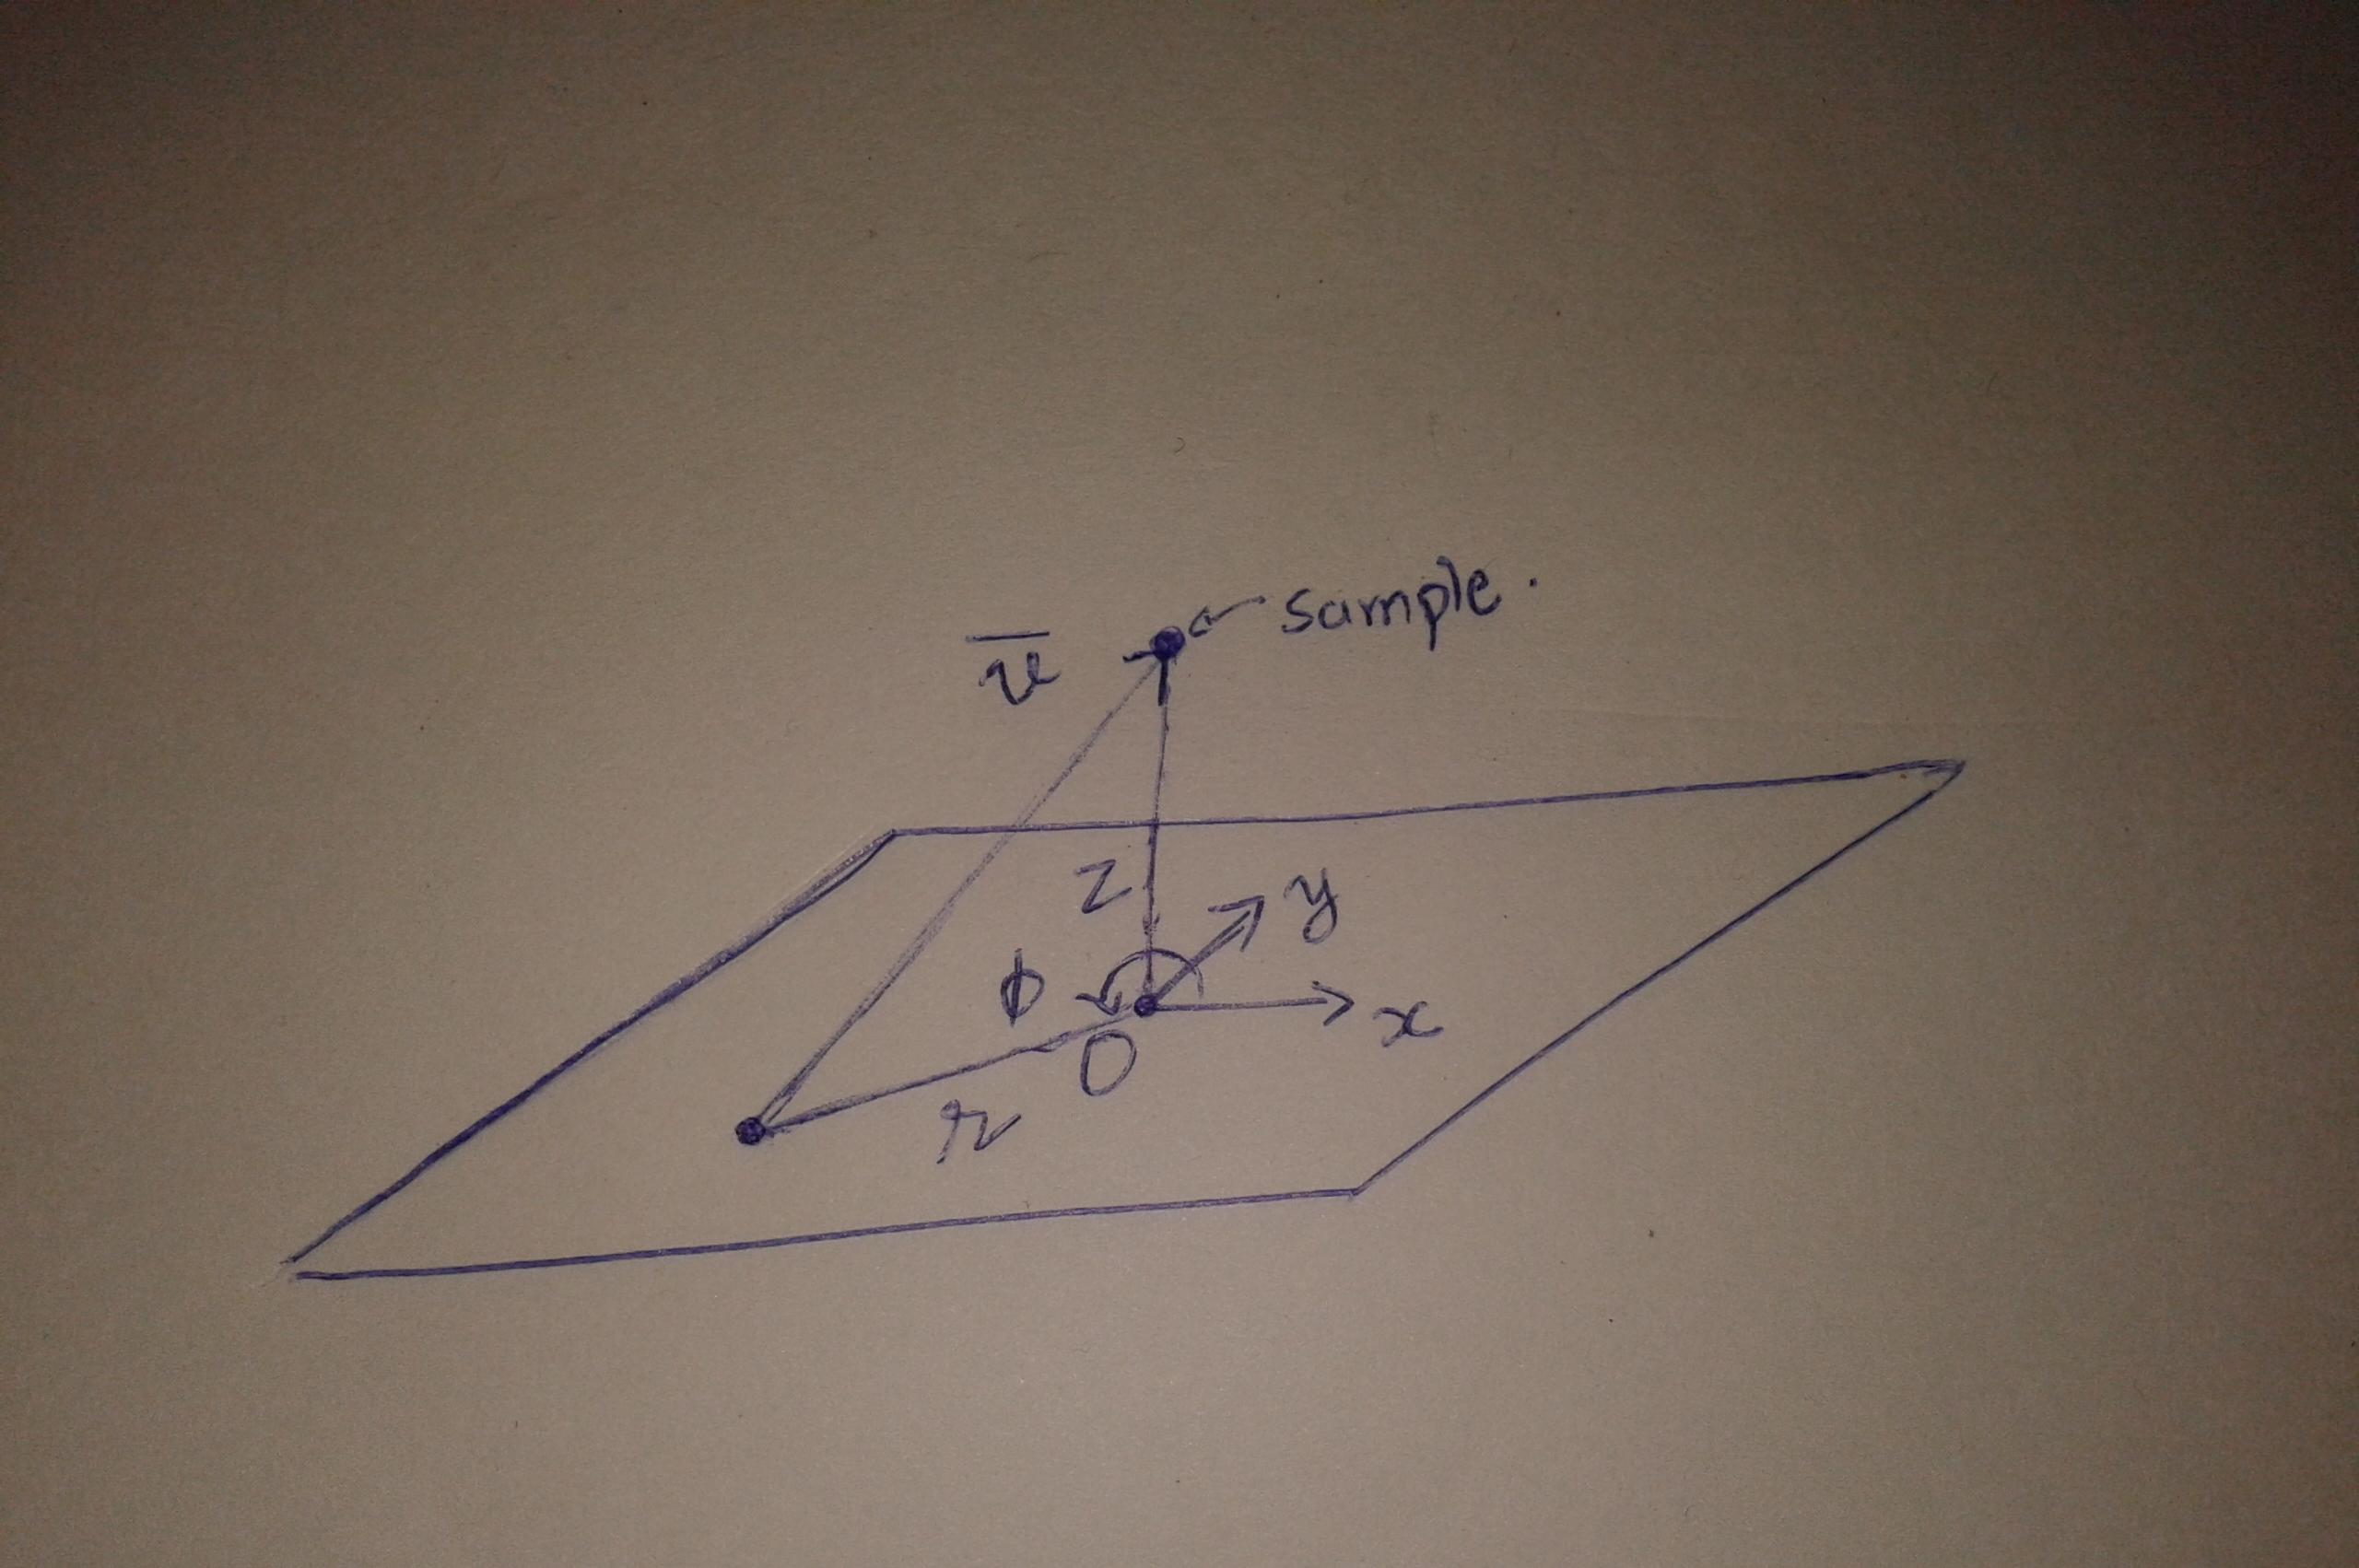
\includegraphics[scale=0.15]{figure.jpg}}

Here an LED at polar coordinates $(r, \phi )$ illuminates the sample. We have to find the illumination angles which give us the direction of the \textit{k} vector and hence $k_x$ and $k_y$. \\

\section{Perfect case of a point sample}

The vector $\vec{v}$ from the LED to the sample may be written as

\begin{equation*} \label{eq1}
\begin{split}
\vec{v} & = (0, 0, z) - (r cos \phi , r sin \phi , 0) \\
 & = -r cos \phi \hat{x} - r sin \phi \hat{y} + z \hat{z}
\end{split}
\end{equation*}

\begin{equation*}
|\vec{v}| = \sqrt{r^2 + z^2}
\end{equation*}

We know $|\vec{k}| = \frac{2 \pi}{\lambda}$, so we get

\begin{equation*}
\vec{k} = \frac{2 \pi}{\lambda} \frac{-r cos \phi \hat{x} - r sin \phi \hat{y} + z \hat{z}}{\sqrt{r^2 + z^2}}
\end{equation*}

yielding

\begin{equation*}
k_x = \frac{-2 \pi r cos \phi}{\lambda\sqrt{r^2 + z^2}}
\end{equation*}

\begin{equation*}
k_y = \frac{-2 \pi r sin \phi}{\lambda\sqrt{r^2 + z^2}}
\end{equation*}

Since the image plane has the same $x$ and $y$ axes as the LED matrix, these $k_x$ and $k_y$ values hold for the image plane as well. \pagebreak

\section{Errors because of dimensions of sample}
In this case, we consider a point on the sample displaced by $(r_e cos \phi , r_e sin \phi, -z_e)$. Under this condition, we need to make sure this point does not go beyond the lens system's transfer function radius, if we want it to be imaged (and want it to count in the image). This will give a constraint on the size of the sample imaged and (a lower bound on) distance z, and `depth' of the sample $z_e$. I'm assuming LED dispersion is sufficient, and the LED is aligned to illuminate the sample. I'm calculating only the lower bound here since we would want the LEDs as close to the sample as possible.

Thus we need the Fourier space distance between the new $k_{x, e}$ and $k_{y, e}$ and the old $k_x$ and $k_y$ less than $\frac{2 \pi NA}{\lambda}$, with NA being the numerical aperture of the imaging lens.

\begin{equation*}
\vec{k} = \frac{2\pi}{\lambda}\frac{(r_e cos \phi_e -r cos \phi) \hat{x} +(r_e sin \phi_e - r sin \phi) \hat{y} + (z-z_e) \hat{z}}{\sqrt{r^2 + z^2}} \left(1+\frac{rr_ecos(\phi - \phi _e)+zz_e}{r^2+z^2}\right)
\end{equation*}
with $r_e << r$, using a first order approximation.

Thus, the changes are
\begin{equation*}
|\Delta k_x| = \frac{2 \pi}{\lambda \sqrt{r^2+z^2}} \left(r_e cos \phi _e - \frac{r cos \phi }{r^2+z^2} (rr_e cos(\phi - \phi _e)+zz_e)\right)
\end{equation*}

\begin{equation*}
|\Delta k_y| = \frac{2 \pi}{\lambda \sqrt{r^2+z^2}} \left(r_e sin \phi _e - \frac{r sin \phi }{r^2+z^2} (rr_e cos(\phi - \phi _e)+zz_e)\right)
\end{equation*}

This implies, 

\begin{equation*}
|\Delta k_f| = \sqrt{|\Delta k_x|^2 + |\Delta k_y|^2} \leq \frac{2 \pi NA}{\lambda}
\end{equation*}

(This seems to be a very tedious calculation and it makes more sense to put in numbers at this step itself.)

\end{document}